%% APPENDIX
%% Can HIV epidemics among men who have sex with men in the Parisian region be eliminated through participation to PrEP rollouts?
%%
%% Jijon S., Molina J.-M., Costagliola D., Supervie V. and Breban R.
%%
%% Paris, October 2020
%%%%%%%%%%%%%%%%%%%%%%%%%%%%%%%%%%%%
\documentclass[11pt]{article}
\usepackage[a4paper,hmargin=2.5cm,vmargin=2.5cm]{geometry}
\usepackage[latin9]{inputenc}
\usepackage[T1]{fontenc} 
\usepackage[english]{babel}
\usepackage{amsmath,amssymb,amsthm}
\usepackage{mathrsfs}											% \rm
\usepackage[hidelinks]{hyperref}
\usepackage[usenames,dvipsnames,table]{xcolor}
\usepackage{graphicx,float}										% Figures
\usepackage{authblk}											% Authors and affiliations
\usepackage[noadjust,super]{cite}									% Bibliography
\usepackage[labelfont=bf,width=\textwidth,nooneline,normalsize]{caption} 	% Caption format
\usepackage{booktabs,multirow}

% Change titles in the ToC
\addto\captionsenglish{\renewcommand{\contentsname}{Table of contents}}
\addto\captionsenglish{\renewcommand{\listfigurename}{Supplementary figures}}
\addto\captionsenglish{\renewcommand{\listtablename}{Supplementary tables}}
% Enumerate elements with an S before the number
\renewcommand{\thesection}{S\arabic{section}}
\renewcommand{\theequation}{S\arabic{equation}}
\renewcommand{\thetable}{S\arabic{table}}
\renewcommand{\thefigure}{S\arabic{figure}}
%%%%%%%%%%%%%%%%%%%%%%%%%%%%%%%%%%%%

\begin{document}

%%
%%	TITLE
%%
%\title{\underline{Appendix}\\ \bigskip
\title{\underline{Supplementary Material}\\ \bigskip
%\title{\underline{Additional file}\\ \bigskip
\LARGE
Can HIV epidemics among men who have sex with men be eliminated through participation to PrEP rollouts? 
}

\author[1]{Sof\'ia Jij\'on}%\thanks{Corresponding author (sofia.jijon@iplesp.upmc.fr)}}
\author[2]{Jean-Michel Molina}%\thanks{jean-michel.molina@aphp.fr}}
\author[1]{Dominique Costagliola}%\thanks{dominique.costagliola@iplesp.upmc.fr}}
\author[1]{Virginie Supervie}%\thanks{virginie.supervie@inserm.fr}}
\author[,3]{Romulus Breban\thanks{Corresponding author (romulus.breban@pasteur.fr)}}

\affil[1]{\small Sorbonne Universit\'e, INSERM, Institut Pierre Louis d'\'Epid\'emiologie et de Sant\'e Publique (UMR-S~1136 IPLESP), F75012 Paris, France.}
\affil[2]{D\'epartement de Maladies Infectieuses, APHP-H\^opital Saint Louis, UMR~941 Inserm et Sorbonne Paris Cit\'e, Paris, France.}
\affil[3]{Institut Pasteur, Unit\'e d'\'Epid\'emiologie des Maladies Emergentes, F75015 Paris, France.}


\date{}

\maketitle

%%
%%	TABLE OF CONTENTS
%%
\newpage
\tableofcontents

\newpage
\listoftables
\listoffigures

%%
%%	SECTION 1. MODEL DESCRIPTION
%%
\newpage
\section{Model description}

We propose a hybrid mathematical model describing the interplay between the HIV epidemic among men who have sex with men (MSM), and individual-level decision-making on whether or not to adopt pre-exposure prophylaxis (PrEP) against HIV infection, in the current therapeutic context, where efficient antiretroviral treatment (ART) is available. We used a deterministic compartmental model to describe HIV transmission among MSM and a game-theoretical approach to model individual's decision-making about PrEP adoption.


\subsection{Modeling the population-level spread of an HIV epidemic}
\subsubsection{Compartmental model without PrEP}

We stratified the MSM population into two risk groups (low and high) to account for heterogeneity in sexual activity and risk of acquiring HIV \cite{Jacquez1989}; we used the subscript $i\in\{h,\ell\}$ ($h$ stands for high and $\ell$ stands for low) to denote these two populations. Furthermore, we assumed that individuals at high risk of infection drive the epidemic, and thus there would be no epidemic if all individuals would be at low risk of HIV infection. 
		
The flow diagram of the HIV epidemic model is shown in figure~\ref{fig:FlowDiag}. Uninfected MSM join the sexually-mixing population at a rate $\pi_i$. Susceptible individuals, $S_i$, get infected with HIV at a rate $\Lambda_i$, which represents the per-capita force of infection; see section \ref{sec:ForceInf} for the definition. Once infected, individuals enter the acute stage of infection and progress to the chronic stage of infection at a rate $\sigma$. We used the superscript $k\in \{a,c\}$ ($a$ stands for acute and $c$ stands for chronic) to distinguish between the stages of infection. Infected individuals, $I_i^k$, are diagnosed at a rate $\theta$, in any stage of infection, and immediately start ART, no longer transmitting HIV \cite{Rodger2016}. That is, only infected individuals unaware of their status transmit HIV. MSM on ART, $T_i$, remain stratified by risk group. Susceptible and undiagnosed MSM spend $1/\mu$ years selecting new sexual partners, while MSM on ART leave the sexually-mixing population at a higher rate, $\mu_T > \mu$. 

The system of ordinary differential equations (ODE) for the HIV epidemic model is the following
\begin{equation} \label{eq:ODEsys}
\begin{aligned}
        dS_i/dt 		& = \pi_i - \left( \Lambda_i + \mu \right) S_i, \\ 
        dI_i^a/dt 		& = \Lambda_i S_i - \left( \sigma + \theta + \mu \right) I_i^a, \\
        dI_i^c/dt 		& = \sigma I_i^a - (\theta +\mu) I_i^c, \\
        dT_i/dt 		& = \theta \left(I_i^a + I_i^c \right) - \mu_T T_i,
\end{aligned}
\end{equation}
where $i \in\{h,\ell\}$. All the variables and parameters are positively defined. The total number of individuals in each risk group is $N_i = S_i + I_i^a + I_i^c + T_i$, and the total population is $N = \sum_i N_i$. 


\subsubsection{Structured mixing}

We consider that individuals do not mix uniformly random (i.e., according to the law of mass action), rather that most partnerships occur within the same risk group (i.e., non-random mixing) 
\cite{Jacquez1988,Koopman1988,Jacquez1989,Gupta1989}. We used $\rho_{ij}$ to denote the probability for an $i$-risk individual to start a sexual partnership with an $j$-risk individual. The matrix
\begin{equation}
\rho= \left(
	\begin{array}{cccc}
	  	\rho_{h h}  	& \rho_{h \ell} \\
	  	\rho_{\ell h} 	& \rho_{\ell \ell} \\
	\end{array}
\right)
\end{equation}
is called {\it mixing matrix}, and its elements verify $0 < \rho_{ij} < 1$ and $\sum_j \rho_{ij} =1$. Since we assumed that individuals mix preferentially within the same risk group, we have $\rho_{ii} > 1/2$. 

We further consider that $i$-risk individuals have $c_i$ new sexual partners per year, and that the number of partners for high-risk individuals was higher than that for low-risk individuals ($c_h > c_\ell $). The total number of partnerships that $i$-risk individuals have with $j$-risk individuals per unit of time is given by $\rho_{ij} c_i N_i$. To balance the total number of partnerships\cite{Jacquez1989}, we require $\rho_{ij} c_i N_i = \rho_{ji} c_j N_j$, which yields
\begin{equation}
	\rho_{\ell h} = (1-\rho_{h h}) \frac{c_h N_h}{c_\ell N_\ell}.
\end{equation}
Furthermore, $\rho_{ii} > 1/2$ yields
\begin{equation} \label{eq:c_h}
	c_h < \frac{c_\ell N_\ell}{2 (1-\rho_{hh})N_h},
\end{equation}
which is an important constraint for the model calibration; see section \ref{sec:Calibration}. In simulations, we assumed that the elements of the mixing matrix remain constant, taking the values obtained through calibration.


\subsubsection{The force of infection} \label{sec:ForceInf}

We use $\beta_j^{k}$ to denote the per-partnership probability of HIV transmission from a $j$-risk infected individual in stage of infection $k$. We reasonably assume that individuals in the acute stage of infection are more likely to transmit HIV than individuals in the chronic stage,\cite{Patel2014} and therefore set $\beta_j^a = w \beta_j^c$, with $w>1$. 

The rate at which $i$-risk susceptibles acquire HIV by forming sexual partnerships with infected individuals is called the {\it force of infection} \cite{Jacquez1988} and is given by
\begin{equation}
	\Lambda_i	 \equiv \sum_{\substack{j \in \{h,\ell\} \\ k\in\{a,c\}}} \frac{c_i \rho_{ij} \beta_j^k I_j^k}{N_j}.
\end{equation}


\subsection{Accounting for the uptake of PrEP}
\subsubsection{Including PrEP epidemiology into the HIV epidemic model} \label{sec:CompartModelPrEP}

We adapt the HIV epidemic model \eqref{eq:ODEsys} for the context where PrEP is available as an HIV prevention method. We suppose that only susceptible individuals having high risk of acquiring HIV are eligible to adopt PrEP. We do not consider that individuals go on and off PrEP, rather that they rigorously follow the PrEP regimen for the entire duration of their sexually mixing period. This modeling choice is further discussed in section~\ref{sec:DecisionMaking}, as it matches other modeling choices for the decision-making game model for the adoption of PrEP. We use $p$ and $\varepsilon$ to denote, respectively, the PrEP coverage and the PrEP effectiveness. Of note, the PrEP coverage parameter is not imposed, rather, it is obtained by solving the decision-making model; see section \ref{sec:DecisionModel}. We assume that individuals on PrEP ($P$) can get infected at a rate $(1-\varepsilon)\Lambda_P$, defined in section~\ref{sec:RiskCompensation}, and get tested for HIV at a rate $\theta_P$. The ODE system of the HIV epidemic model becomes
\begin{equation} \label{eq:ODEsysP} 
\begin{aligned}
        dP/dt 		& = p \pi_h - \Big( (1-\varepsilon) \Lambda_P + \mu \Big) P, \\
        dS_h/dt 		& = (1-p) \pi_h - \left( \Lambda_h + \mu \right) S_h, \\ 
        dS_\ell/dt 		& = \pi_\ell - \left( \Lambda_\ell + \mu \right) S_\ell, \\ 
        dI_P^a/dt		& = (1-\varepsilon) \Lambda_P P - \left(\sigma + \theta_P + \mu \right) I_P^a, \\
        dI_h^a/dt 		& = \Lambda_h S_h - \left( \sigma + \theta + \mu \right) I_h^a, \\
        dI_\ell^a/dt 	& = \Lambda_\ell S_\ell - \left( \sigma + \theta + \mu \right) I_\ell^a, \\
        dI_P^c/dt 		& = \sigma I_P^a - \left( \theta_P + \mu \right) I_P^a,\\
        dI_h^c/dt 		& = \sigma I_h^a - (\theta +\mu) I_h^c, \\
        dI_\ell^c/dt 	& = \sigma I_\ell^a - (\theta +\mu) I_\ell^c, \\
        dT_h/dt 		& = \theta_P \left( I_P^a + I_P^c\right) + \theta \left(I_h^a + I_h^c \right) - \mu_T T_h, \\
        dT_\ell/dt 		& = \theta \left(I_\ell^a + I_\ell^c\right) - \mu_T T_\ell,
\end{aligned}
\end{equation}
illustrated by the flow diagram in figure~\ref{fig:FlowDiagP}. The ODE system~\eqref{eq:ODEsysP} has two equilibria: an endemic state (ES) where all the population compartments are non-empty, and a disease-free state (DFS) with no infected individuals
\begin{equation}
	I_i^{k,\rm DFS} = 0,\quad T_i^{\rm DFS} = 0, \qquad \text{for all } i\in\{P,h,\ell\}, \, k\in\{a,c\},
\end{equation}
only uninfected individuals, whether or not on PrEP
\begin{equation}
	P^{\rm DFS}\neq 0,\quad S_i^{\rm DFS}\neq 0, \qquad \text{for all } i\in\{h,\ell\}.
\end{equation}

We further assume that the per-partnership probability for acquiring HIV from an infected, high-risk MSM is the same, whether or not the MSM is taking PrEP. Hence, the force of infection for the population at $i$-risk of infection, not taking PrEP, becomes
\begin{equation}
	\Lambda_i	 = c_i \left( \frac{\rho_{ih} \beta_h^a \big(I_P^a + I_h^a\big) + \rho_{ih} \beta_h^c \big(I_P^c +I_h^c \big)}{N_h} + \frac{\rho_{i\ell} \beta_\ell^a I_\ell^a + \rho_{i\ell} \beta_\ell^c I_\ell^c}{N_\ell}\right), \quad \text{for } i \in\{h,\ell\},
\end{equation}
where
\begin{equation}
N_h = P + S_h + I_P^a + I_P^c + I_h^a + I_h^c + T_h,
\end{equation}
and
\begin{equation}
N_\ell = S_\ell + I_\ell^ a + I_\ell^c + T_\ell.
\end{equation}


\subsubsection{PrEP-induced risk compensation} \label{sec:RiskCompensation}

The PREVENIR study reported that MSM using PrEP may use condoms less often \cite{Molina2018}; we call this the phenomenon of {\it risk compensation}. We model risk compensation among susceptibles on PrEP explicitly, showing how the force of infection for high-risk susceptibles on PrEP depends on condom effectiveness and condom use among high-risk susceptibles.

We denote by $\beta_{jh}^k$ the per-partnership probability of HIV transmission from a $j$-risk individual in $k$ stage of infection toward high-risk susceptibles. This can be written as
 \begin{equation}
 	\beta_{jh}^k \equiv \beta_{j 0}^k(1-\xi \eta_h) = \beta_j^k,
 \end{equation}
where $\beta_{j 0}^k$ is the baseline (i.e., without condom) per-partnership probability, $\xi$ denotes condom effectiveness and $\eta_h$ is the probability of using condoms for high-risk susceptibles before the introduction of PrEP.

We assumed that, once PrEP becomes available, high-risk susceptibles, who do not adopt PrEP, continue to use condoms with probability $\eta_h$, while high-risk susceptibles who adopt PrEP use condoms with probability $\eta_P < \eta_h$; i.e., they are less likely to use condoms. We thus obtained that the per-partnership probability of HIV transmission to high-risk susceptibles on PrEP is given by $\beta_j^k (1-\xi \eta_P)/(1-\xi \eta_h)$. In sum, the force of infection on high-risk susceptibles taking PrEP is given by
\begin{equation}
	(1-\varepsilon) \Lambda_P = (1-\varepsilon) \left(\frac{1-\xi \eta_P}{1-\xi \eta_h}\right) \Lambda_h.
\end{equation}


\subsubsection{The effective reproduction number}

We computed the {\it effective reproduction number} for the ODE system~\eqref{eq:ODEsysP}, the expected number of secondary cases produced by a single infected individual, during his entire infectious period, in an uninfected population subject to control interventions \cite{Anderson1991,VanDenDriessche2008}, and we expressed it as a function of the PrEP coverage and effectiveness

\begin{equation}
	R(p,\varepsilon) = A \left[ H(p,\varepsilon) + M + \sqrt{ \Big(H(p,\varepsilon) - M\Big)^2 + 4 B H(p,\varepsilon) M }\,\right],
\end{equation}
where 
\begin{align} 
	& A^{-1} \equiv \, 2 (\theta+\mu) (\theta_P+\mu) (\sigma+\theta+\mu) (\sigma+\theta_P+\mu),\\
	& B \equiv \, \left(\frac{1}{\rho_{h h}}-1\right) \left(\frac{1}{\rho_{\ell \ell}}-1\right),\\
	& M \equiv \, (\theta_P+\mu) (\sigma+\theta_P+\mu) \Big[(\theta+\mu) c_\ell \rho_{\ell \ell}\beta_\ell^a+\sigma c_\ell \rho_{\ell \ell}\beta_\ell^c\Big], \end{align}
are independent of the PrEP parameters. In contrast, $H(p,\varepsilon)$ is the following function of $p$ and $\varepsilon$
\begin{equation}
	H(p,\varepsilon) \equiv \, (1-p) H_h + p (1-\varepsilon) \left( \frac{1-\xi \eta_P}{1-\xi \eta_h}\right) H_P,
\end{equation}
where
\begin{equation}
H_h \equiv (\theta_P+\mu) (\sigma+\theta_P+\mu) \Big[ (\theta+\mu) c_h \rho_{hh} \beta_h^a + \sigma c_h \rho_{hh} \beta_h^c \Big],
\end{equation}
and
\begin{equation}
H_P \equiv (\theta+\mu) (\sigma+\theta+\mu) \Big[ (\theta_P+\mu) c_h \rho_{hh} \beta_h^a + \sigma c_h \rho_{hh} \beta_h^c\Big],
\end{equation}
do not depend on PrEP parameters

We used the effective reproduction number to quantify the impact of PrEP on the HIV epidemic. We refer to the epidemic as being {\it controlled by PrEP} if the effective reproduction number after the introduction of PrEP is lower than that in the absence of PrEP; i.e., if $R(p,\varepsilon) < R(0,\varepsilon)$. A transcritical bifurcation occurs for the ODE system~\eqref{eq:ODEsysP} when $R(p,\varepsilon)=1$ \cite{Jacquez1988,VanDenDriessche2008}. If $R(p,\varepsilon)>1$, then the endemic state will be reached; if $R(p,\varepsilon) < 1$ then the disease-free state will be reached. We say the epidemic among MSM is {\it eliminated by PrEP} if $R(p,\varepsilon) \leq 1$. 

It is important to note that the introduction of PrEP does not lead unconditionally to control of the HIV epidemic, especially that the introduction of PrEP can cause less condom use. In the following of this manuscript, we determine the conditions for which PrEP prevention can induce control and elimination of the HIV epidemic.


\paragraph{The epidemic control threshold.} 

For the epidemic to be controlled, certain conditions for PrEP uptake, HIV testing and condom use parameters must be satisfied. In particular, we found a threshold value for the PrEP effectiveness, denoted $\varepsilon_{\rm C}$, ensuring $R(p,\varepsilon) < R(0,\varepsilon)$ if and only if $\varepsilon \geq \varepsilon_{\rm C}$, where
\begin{equation}
	\varepsilon_{\rm C}\equiv 1 - \left( \frac{1-\xi \eta_h}{1-\xi \eta_P}\right) \left(\frac{H_h}{H_P}\right).
\end{equation}


\paragraph{The epidemic elimination threshold.} 

In our model, epidemic elimination (i.e., $R(p,\varepsilon) \leq 1$) is possible if and only if the {\it effective PrEP coverage}, $\varphi(\varepsilon) \, p$, is equal to or larger than $K$, where 
\begin{equation}
	\varphi(\varepsilon) \equiv H_h - (1-\varepsilon) \left( \frac{1-\xi \eta_P}{1-\xi \eta_h}\right) H_P.
\end{equation} 
and $K$ is a constant independent of the PrEP parameters defined by
\begin{equation}
	K \equiv H_h - \left(M - \frac{1}{2A}\right) \left(\frac{1}{2AM (1-B) -1}\right).
\end{equation}

The lowest value for the PrEP effectiveness allowing for the HIV epidemic elimination is obtained assuming full PrEP coverage: $R(p=1,\varepsilon) \leq 1$ if and only if $\varepsilon\geq\varepsilon_{\rm E}$, where
\begin{equation}
	\varepsilon_{\rm E} \equiv 1- \left( 1- \frac{K}{H_h}\right) (1-\varepsilon_{\rm C}).
\end{equation}
Hence, the epidemic elimination condition $R(p,\varepsilon) \leq 1$ is met when $\varphi(\varepsilon) \, p \geq K$, for  $\varepsilon\geq\varepsilon_{\rm E}$ and $0\leq p\leq 1$.


\subsection{Modeling individual-level decision-making on PrEP adoption} \label{sec:DecisionMaking}
\subsubsection{Decision model} \label{sec:DecisionModel}

We propose a mathematical model for the individual-level decision-making on whether or not to adopt PrEP for HIV prevention. As mentioned in section~\ref{sec:CompartModelPrEP}, we assume that only uninfected individuals at high risk of infection are proposed to adopt PrEP. 

We use a game-theoretical approach, where individuals act alone and in their own interest. Individuals are considered to weigh their perceived pros and cons of using PrEP, versus getting infected and the consequent lifelong ART. These pros and cons consist of monetary and/or non-monetary aspects such as: undesired secondary effects, price, reimbursement policies, accessibility, social stigma, disease morbidity, etc.\cite{Arnold2016,Gilson2018,Thomann2017,Brooks2019}. Pros and cons are expressed as {\it costs} perceived by the individual and they are balanced in a {\it utility function}. Then, the individual-level decision-making on whether or not to adopt PrEP is modeled by the maximization of the utility, which is equivalent to the minimization of the total expected cost by the individual MSM.

The solution of the game model is an equilibrium situation for the HIV epidemiology, where a fraction of the individuals adopt PrEP in stationary epidemic conditions; i.e.~there are no longer changes in prevention behavior. We therefore assumed that, in the long term, the individuals are pleased with their decision regarding PrEP adoption, which they maintain for the duration of their sexually mixing period. That is, we do not model changes of decision and recurrent decision-making. In addition, we consider no formal difference between PrEP regimens (daily or event-driven PrEP approach).  


\subsubsection{Utility of PrEP for the individual-level decision-making} \label{sec:Utility}

An individual at high risk of infection can adopt one of the two mutually exclusive strategies: not to use PrEP, at a perceived cost $C_{\text{\tiny No-PrEP}}>0$ or to use PrEP for HIV prevention, at a perceived cost $C_{\text{\tiny PrEP}}>0$. For a probability $p$ to adopt PrEP, the expected utility $U(p)$ for the individual is given by 

\begin{equation}
	U(p) = - p \, C_{\text{\tiny PrEP}} - (1- p) \, C_{\text{\tiny No-PrEP}}\equiv-C(p), 
\end{equation}
where $C(p)$ stands for the total expected cost.

\paragraph{The cost of adopting the strategy of not using PrEP.}

In the case where an individual decides not to use PrEP, he may get infected, starts treatment upon positive HIV diagnosis, and eventually pays the cost of ART for the rest of his life. We thus assumed that an individual who decides not to use PrEP pays, once he becomes HIV infected during his sexually-mixing period, the cost of ART. After leaving the sexually-mixing population, if infected with HIV, the individual continues to pay the cost of ART for the rest of his life. An individual who decides not to use PrEP and does not get infected with HIV pays no cost. Mathematically, the cost of adopting the strategy of not using PrEP can be written as

\begin{equation} \label{eq:C_NoPrEP}
	C_{\text{\tiny No-PrEP}}(p,\varepsilon) \equiv \int_ 0^{L} \left(1- e^{-\lambda(p,\varepsilon) t} \right) c_T \,dt + \int_L^{L+L_T} \left(1- e^{-\lambda(p,\varepsilon) L} \right) c_T \,dt,
\end{equation}
where $c_T$ is the per-year perceived cost of ART, $L$ is the number of years that an infected individual stays sexually mixing,  $L_T$ is the number of life years remaining after leaving the sexually-mixing population for individuals on ART, $\lambda$ is the rate of getting infected with HIV; see section~\ref{sec:PerceivedRisk}.

\paragraph{The cost of adopting the strategy of using PrEP to avoid HIV infection.}

Similarly, in the case where an individual decides to adopt PrEP, he would take and pay the cost of PrEP and, in the case of acquiring HIV despite PrEP uptake, being diagnosed and starting ART, he would pay the cost of treatment for the rest of his life. This is summarized mathematically as follows
\begin{equation} \label{eq:C_PrEP}
	C_{\text{\tiny PrEP}}(p,\varepsilon) \equiv \int_ 0^{L} e^{-\lambda_P(p,\varepsilon) t} c_P \,dt + \int_ 0^{L} \left(1- e^{-\lambda_P(p,\varepsilon) t} \right) c_T \,dt + \int_L^{L+L_T} \left(1- e^{-\lambda_P(p,\varepsilon) L} \right) c_T \,dt,
\end{equation}
where $c_P$ is the per-year perceived cost of PrEP and $\lambda_P$ is the rate of getting infected with HIV despite taking PrEP; see section~\ref{sec:PerceivedRisk}. \\

We introduce the {\it relative cost of prevention versus treatment} (i.e., PrEP versus ART), $r = c_P/c_T>0$. Rescaling equations~\eqref{eq:C_NoPrEP} and~\eqref{eq:C_PrEP} by $c_T$ and maintaining the notation (namely, keeping the symbols $C_{\text{\tiny No-PrEP}}$, $C_{\text{\tiny PrEP}}$ and $U$ for the rescaled quantities), we rewrite the utility function as follows:
\begin{equation}
	U(p;\varepsilon, r) = - p \, C_{\text{\tiny PrEP}}(p;\varepsilon, r) - (1- p) \, C_{\text{\tiny No-PrEP}}(p;\varepsilon)\equiv-C(p;\varepsilon, r).
\end{equation}

The PrEP coverage that maximizes $U(p;\varepsilon, r)$ or, equivalently, minimizes the expected cost $C(p;\varepsilon, r)$ is interpreted as the probability of an MSM at high risk of infection to use PrEP, which yields the {\it voluntary PrEP coverage}, $\hat{p}(\varepsilon,r)$, as a function of PrEP effectiveness, $\varepsilon$, and the relative cost of PrEP versus ART, $r$. 


\subsubsection{Risk of HIV infection perceived by high-risk individuals} \label{sec:PerceivedRisk}

In the baseline scenario, we assumed that individuals have a fair sense of their own risk to acquire HIV. Thus, in the absence of an HIV epidemic, individuals (whether or not on PrEP) acknowledge zero risk; that is,
\begin{equation}
	\Lambda_h^{\rm DFS}=\Lambda_P^{\rm DFS}=0.
\end{equation} 

In the case of adopting the No-PrEP strategy, individuals acknowledge a risk of infection given by the force of infection for high-risk individuals not on PrEP, at the endemic state,
\begin{equation}
	\Lambda_h^{\rm ES}(p,\varepsilon) = c_h \left( \frac{\rho_{ih} \beta_h^a \Big(I_P^{a,\rm ES} + I_h^{a,\rm ES}\Big) + \rho_{ih} \beta_h^c \Big(I_P^{c,\rm ES} +I_h^{c,\rm ES} \Big)}{N_h^{\rm ES}} + \frac{\rho_{i\ell} \beta_\ell^a I_\ell^{a,\rm ES} + \rho_{i\ell} \beta_\ell^c I_\ell^{c,\rm ES}}{N_\ell^{\rm ES}}\right),
\end{equation}
where the population variables $I_j^{k,\rm ES}$, for $j\in\{P,h,\ell\}$, $k\in\{a,c\}$ and $N_j^{\rm ES}$, for $i\in\{h,\ell\}$ depend implicitly on $p$ and $\varepsilon$. In the case of adopting PrEP, individuals acknowledge a risk of infection given by the force of infection for high-risk individuals on PrEP at the endemic state
\begin{equation} \label{eq:Lambda_P_ES}
	(1-\varepsilon) \Lambda_P^{\rm ES}(p,\varepsilon) = (1-\varepsilon) \left(\frac{1-\xi \eta_P}{1-\xi \eta_h}\right)\Lambda_h^{\rm ES}(p,\varepsilon).
\end{equation} 

Specifically, $\lambda(p,\varepsilon)$, the rate of HIV infection for individuals, who decide not to use PrEP, is given by
\begin{equation}
	\lambda (p,\varepsilon) = \left\{
	\begin{aligned}
		&\Lambda_h^{\rm ES}(p,\varepsilon),& \quad \text{if } R(p,\varepsilon)>1,\\
		&\Lambda_h^{\rm DFS}, & \quad \text{if } R(p,\varepsilon)\leq 1;
	\end{aligned}
	\right.
\end{equation}
while $\lambda_P$, the rate of becoming infected despite taking PrEP for individuals who decide to use PrEP (cf. equation~\eqref{eq:C_PrEP}), is given by
\begin{equation} \label{eq:lambda_P}
	\lambda_P (p,\varepsilon) = \left\{
	\begin{aligned}
		&(1-\varepsilon)\Lambda_P^{\rm ES}(p,\varepsilon),& \quad \text{if } R(p,\varepsilon)>1,\\
		&\Lambda_P^{\rm DFS}, & \quad \text{if } R(p,\varepsilon)\leq 1.
	\end{aligned}
	\right.
\end{equation}
The quantities $\lambda(p,\varepsilon)$ and $\lambda_P(p,\varepsilon)$ are used in the definitions of $C_{\text{\tiny PrEP}}(p;\varepsilon, r)$ and $C_{\text{\tiny No-PrEP}}(p;\varepsilon)$, the perceived costs for the strategies to adopt PrEP and not to adopt PrEP, respectively; see section \ref{sec:Utility}.


%%
%%	SECTION 2. CALIBRATION
%%
\newpage
\section{Model calibration} \label{sec:Calibration}

The hybrid model combining the ODE system and the decision model was built in MATLAB (release 2018). We first calibrated the model~\eqref{eq:ODEsys} to reproduce the HIV epidemiology among MSM in the Paris region, \^Ile-de-France, assumed to be close to an endemic state in 2016~\cite{RapportSPF2019}. The initial values used for the HIV transmission parameters in the calibration process are listed in tables~\ref{tab:InitConds} and~\ref{tab:Params}, respectively. As calibration criteria, we used estimates for MSM in \^Ile-de-France, listed in table~\ref{tab:Calibration}, regarding the HIV incidence rate, prevalence of undiagnosed infections \cite{Marty2019}, prevalence of HIV \cite{Prevagay2017}, size of the MSM population \cite{Bajos2018,Insee2015}; we used the HIV incidence estimated by the ANRS IPERGAY study in Paris \cite{Molina2018} as an upper bound for the incidence among high-risk MSM. The epidemiological indicators were related to model simulations according to the formulae given in table~\ref{tab:EpiIndFormulas}. 

Using the initial ranges (cf. tables~\ref{tab:InitConds} and~\ref{tab:Params}), we generated 500\,000 parameter sets through latin hypercube sampling, assuming that each parameter follows a uniform distribution. Out of these 500\,000 parameter sets, $111$ passed the calibration checks. Then, to refine the calibration, we generated additional $1\,400$ parameters sets, by sampling nearby the previously obtained parameter sets. In total, $505$ parameter sets passed the calibration checks. Summary statistics for each HIV parameter yields a mean and a 95\% confidence interval (CI); see table~\ref{tab:Params}.  Of note, that the calibration selects for $\beta^k_h>\beta^k_\ell$, which, indeed, suggests an intrinsic, riskier behavior for individuals with high sexual activity. 

Using our $\sim500$ calibrated parameter sets, we estimated epidemiological indicators for the HIV epidemic in the MSM community of \^Ile-de-France.  They provide our modeling perspective on the HIV epidemiology before the introduction of PrEP (cf. table~\ref{tab:Calibration}): overall yearly mean incidence was $1.3\%$, mean prevalence $17\%$, and $17\%$ of MSM living with HIV were unaware of their HIV status. The mean number of MSM was $\sim111\,000$, of which $\sim14\,200$ were at high risk of HIV infection and eligible for PrEP. Yearly mean HIV incidence for high-risk MSM was $7\%$. We note, however, that our estimates for the HIV epidemiological indicators, resulting from the model calibration, do not differ much from the estimates obtained through direct data analyses (cf. table~\ref{tab:Calibration}), indicative of successful calibration. The $\sim500$ calibrated parameter sets were further used for simulations regarding the introduction of PrEP and the decision model.

%%
%%	SECTION 3. SUPPLEMENTARY RESULTS
%%
%\newpage
\section{Supplementary results}

\subsection{Impact of PrEP rollouts on HIV epidemics}

In France, PrEP prescriptions need to be renewed every three months.\cite{CNSANRS2018} Meanwhile, the PrEP-eligible individual must provide proof that they tested negative for HIV infection. Consequently, on-PrEP MSM get tested for HIV every three months, which determines our parameter $1/\theta_P=3~{\rm months}$; see table~\ref{tab:Params}. It is very important to note that on-PrEP MSM get tested much more frequently than MSM before the PrEP rollout, when the median time from HIV infection to diagnosis for MSM was 3.1 years~\cite{Marty2019}. Due to the dramatic change in testing behavior, the PrEP rollout can act as a test-and-treat intervention, where individuals get tested very often for HIV infection, and start treatment upon positive diagnostic, no longer transmitting HIV. In principle, this can be sufficient to eliminate the HIV epidemic, even without PrEP. \cite{Kretzschmar2013,WHO2016} 

The deterministic component of our HIV model \eqref{eq:ODEsysP} can offer insight into the epidemic-level impact of a PrEP rollout, and the action of various parameters. Figure~\ref{fig:R}A depicts the effective reproduction number $R$ versus $\varepsilon$ and $p$, for one typical parameter set calibrating our model.  According to our baseline scenario, we assumed that high-risk MSM, not taking PrEP, use condom with probability $30\%$, and if they take PrEP, the probability drops at $20\%$; condom effectiveness was considered to be $70\%$. The fact that a $70\%$-$80\%$ PrEP coverage is sufficient to eliminate HIV, even when PrEP efficacy is zero, is entirely due to the test-and-treat effect of the PrEP rollout, as explained before. In particular, this implies that the thresholds in PrEP effectiveness, such that epidemic control and elimination are possible, are zero; i.e., $\varepsilon_{\rm E} = \varepsilon_{\rm C} = 0$. The test-and-treat action of the PrEP rollout is further evidenced in figure~\ref{fig:R}B, which represents $R$ as a function of the PrEP coverage $p$ and testing rate $\theta_P$, assuming that the effectiveness of PrEP is zero ($\varepsilon=0$); that is, there is no PrEP and $p$ is the coverage of frequent testing, with the rate $\theta_P$. Figure~\ref{fig:R}B reveals that, for HIV elimination in the absence of PrEP (i.e., or using a PrEP regimen with no efficacy), it would suffice that $\sim 80\%$ of the high-risk MSM in the Paris region got tested every three months; see figure~\ref{fig:R} for $p=80\%$ and $\theta_P=4~\rm{years^{-1}}$. Still, an intervention based just on the test-and-treat strategy may be difficult to implement. The individual at risk is not directly protected from acquiring HIV, by joining a test-and-treat program. Rather, the benefits are indirect, emerging from the success of the test-and-treat intervention at the population level. It is thus expected that test-and-treat interventions have low acceptability. The French guidelines recommend, since 2009, annual HIV testing for MSM at risk, and 3-month testing since 2017. Yet, testing rate estimates are significantly lower, since the median time from HIV infection to diagnosis for MSM was estimated at 3.1 years.~\cite{Marty2019}

The distinct advantage of PrEP rollouts is that they offer direct protection to individuals at risk of acquiring HIV, through highly effective PrEP regimens. Hence, the individual recognizes his interest in adopting PrEP, and may join the PrEP rollout voluntarily, ensuring high acceptability for PrEP rollouts. Furthermore, as more and more individuals join the prevention effort, population-level benefits emerge, down to HIV elimination.


\subsection{Adoption of PrEP under the baseline scenario}

In the baseline scenario, we assumed that individuals have a fair sense of their risk of infection and condom use drops from 30\% to 20\% when individuals adopt PrEP.\cite{Molina2015} The risk of HIV infection is computed using the HIV transmission model, and corresponds to the force of HIV infection (cf. section~\ref{sec:PerceivedRisk}). 
In addition, we considered that on-PrEP MSM follow the recommendations of the regimen, which requires 3-month testing to renew their PrEP prescription~\cite{Molina2015}. Therefore, MSM on PrEP are advised to test much more frequently than what is the current practice of MSM not taking PrEP; i.e.,~$\theta_P \ll \theta$ and the PrEP rollout can share the action of a test-and-treat intervention. We found that, in this case, the thresholds in PrEP effectiveness, such that epidemic control and elimination are possible, are zero; i.e., $\varepsilon_{\rm E} = \varepsilon_{\rm C} = 0$.


\subsubsection{Voluntary PrEP coverage}

We computed the voluntary PrEP coverage among high-risk MSM, denoted $\hat{p}$, for one typical parameter set calibrating our model; see table~\ref{tab:Params}. The PrEP coverage starts at zero, before the introduction of PrEP, and then reaches an optimal value where the expected cost of adopting PrEP is minimum. The final value reached by $\hat{p}$ depends on HIV epidemic parameters before the introduction of PrEP, that were found by calibration, PrEP effectiveness, $\varepsilon$, and perceived relative cost of PrEP versus ART, $r$, which were varied over broad ranges. 

Our previous work \cite{Jijon2017} helped identify the conditions for which our model algorithms could be reliably implemented. Indeed, if $R(\hat{p},\varepsilon) \leq 1$, then there is no stable~equilibrium for the individual strategies and numerical methods fail to compute an approximation for the voluntary PrEP coverage, $\hat{p}(\varepsilon, r)$; otherwise, numerical estimation of $\hat{p}(\varepsilon, r)$ is possible. We say that, for $R(\hat{p},\varepsilon) \leq 1$, the game regarding the adoption of PrEP has no solution.

As a supplement to the colormaps in figure 1 of the main text, figure~\ref{fig:p_hat} depicts the PrEP coverage reached voluntarily among high-risk MSM, $\hat{p}(\varepsilon,r)$, and the corresponding endemic force of infection among high-risk MSM when the PrEP effectiveness is $\varepsilon=86\%$; n.b., $\hat{\Lambda}_h^{\rm ES}(\varepsilon,r) \equiv \Lambda_h^{\rm ES}\left(\hat{p}(\varepsilon,r),\varepsilon\right)$. For a given value of the PrEP effectiveness, $\varepsilon$, we used $r_{\rm E}(\varepsilon)$ and $r_{\rm C}(\varepsilon)$ to denote, respectively, the elimination and control threshold values for the relative cost; n.b.,~$ 0 < r_{\rm E}(\varepsilon) < r < r_{\rm C}(\varepsilon)$ implies $0\%<\hat{p}(\varepsilon,r)<100\%$. The three regions identified in figure 1 of the main text are also present in figure~\ref{fig:p_hat}, delimited by the thresholds in PrEP effectiveness and relative cost (n.b., $\varepsilon=86\%$ for figure~\ref{fig:p_hat}):

\begin{itemize}
\item Region~III, where $r \geq r_{\rm C}(\varepsilon)$. The relative cost of prevention versus treatment is perceived as being too high. Therefore, no one adopts the strategy of using PrEP to prevent HIV infection (i.e., $\hat{p}(\varepsilon,r)=0\%$) and the endemic state of the epidemic stays unaffected (i.e., $\hat{\Lambda}_h^{\rm ES}(\varepsilon,r) = \Lambda_h^{\rm ES}(0,0)$). 

\item Region~II, where $r_{\rm E}(\varepsilon) < r < r_{\rm C}(\varepsilon)$. The relative cost is low enough, so a proportion of high-risk MSM adopts the strategy of using PrEP (i.e., $0 \%< \hat{p}(\varepsilon,r) <100\%$). However, not enough MSM adopt PrEP and thus, the {\it effective, voluntary PrEP coverage}, $\varphi(\varepsilon) \, \hat{p}(\varepsilon,r)$, is below the threshold $K$. Hence, the HIV epidemic is controlled (i.e., $\hat{\Lambda}_h^{\rm ES}(\varepsilon,r) < \Lambda_h^{\rm ES}(0,0)$), but not eliminated. 

\item Region~I, where $0 \leq r\leq r_{\rm E}(\varepsilon)$. The relative cost is low, and the PrEP effectiveness is above the elimination threshold, thus the effective, voluntary PrEP coverage, $\varphi(\varepsilon) \, \hat{p}(\varepsilon,r)$, may reach or exceed the threshold $K$, so the epidemic may be averted. Hence, in region~I, the reproduction number is below 1 (i.e., $R\left(\hat{p}(\varepsilon,r),\varepsilon\right) \leq 1$).
 \end{itemize}
 
 
\subsubsection{Relative reduction in HIV incidence rate}

The endemic HIV incidence rate reached after the introduction of PrEP (cf. model~\eqref{eq:ODEsysP}) is given by
\begin{equation}
	\mathcal{I}^{\rm ES}(p, \varepsilon) \equiv \frac{(1-\varepsilon) \Lambda_h^{\rm ES} P^{\rm ES} + \Lambda_h^{\rm ES} S_h^{\rm ES} + \Lambda_\ell^{\rm ES} S_\ell^{\rm ES}}{P^{\rm ES} + S_h^{\rm ES} + S_\ell^{\rm ES}}.
\end{equation}

The endemic incidence rate in the absence of PrEP is $\mathcal{I}^{\rm ES}(0, 0) = 1.3\%$. Figure~1B of the main text depicts the relative reduction in the endemic HIV incidence rate due to voluntary PrEP coverage, $ \left[\mathcal{I}^{\rm ES}(0, 0) - \mathcal{I}^{\rm ES}(\hat{p}(\varepsilon,r),r) \right]/\mathcal{I}^{\rm ES}(0, 0)$. Note that increasing PrEP effectiveness and reducing PrEP cost results in greater reduction of the endemic incidence rate, provided that the condition for epidemic control regarding PrEP effectiveness is met; i.e., $\varepsilon > \varepsilon_{\rm C}$.


\subsection{Sensitivity analyses}
\subsubsection{Risk misperception}

In the baseline scenario, we assumed that high-risk MSM have a fair sense of their risk of infection when deciding whether or not to adopt PrEP; this risk of infection was computed using the HIV transmission model, and corresponds to the force of HIV infection; see section~\ref{sec:PerceivedRisk}. However, individuals could misperceive their risk of acquiring infection \cite{Blumenthal2019}.  In a sensitivity scenario, we assumed that individuals underestimate their risk of infection when deciding whether or not to adopt PrEP. Specifically, we assumed that high-risk MSM get a sense of the risk of infection from, for instance, the rate of their high-risk MSM peers being diagnosed with HIV each year, given by
\begin{equation}
	\tilde{\Lambda} (p, \varepsilon) \equiv \frac{\theta_P \left(I_P^{a,\rm ES} + I_P^{c,\rm ES}\right) + \theta \left(I_h^{a,\rm ES} + I_h^{c,\rm ES}\right)}{P^{\rm ES} + S_h^{\rm ES} + I_P^{a,\rm ES} + I_P^{c,\rm ES} + I_h^{a,\rm ES} + I_h^{c,\rm ES}} .
\end{equation}

We repeated our analyses using $\tilde{\Lambda}$ in equations~\eqref{eq:Lambda_P_ES}--\eqref{eq:lambda_P} instead of $\Lambda_h^{\rm ES}$ and compared the results with those of the baseline scenario; see figure~3 of the main text. The HIV epidemiological picture regarding voluntary PrEP coverage is qualitatively similar. That is, we recover the 3-region structure and the voluntary PrEP coverage required for HIV elimination is the same. Still, the misperception of infection risk leaves less room for intervention aiming at epidemic elimination: Region~I gets significantly reduced along the relative cost axis ($r$), compared with the baseline scenario using the force of infection for the perceived risk; see figure~3 of the main text. In particular, for a PrEP effectiveness of 86\%, the cost of PrEP relative to that of ART should be lowered by a factor of $\sim 2$ relative to the baseline scenario, in order to reach Region~I. 

\subsubsection{Condom use and risk compensation}

In the baseline scenario, we assumed that there is a drop in condom use among PrEP users from $\eta_h=30\%$ to $\eta_P=20\%$. In a worse-case scenario for condom drop (i.e., a sensitivity scenario), we considered that individuals on PrEP stop using condoms completely (i.e., $\eta_P=0\%$) and, redoing the analyses, we compared the results with those of the baseline scenario; see figure~\ref{fig:p_hat_CondomDrop}. Risk compensation among PrEP users has low impact on our results: (1) the boundary between regions~II and~III shifts only slightly, and (2) only slightly higher levels of PrEP coverage are required for epidemic elimination when PrEP users completely drop condom use.


\subsubsection{Unchanged rates of HIV testing for individuals on PrEP}

In the baseline scenario, we assumed that on-PrEP MSM test against HIV every 3 months. Here, we considered that on-PrEP MSM do not change their behavior regarding HIV testing; that is, the PrEP program does not require a change in testing behavior, thus $\theta_P=\theta$. Therefore, we have
\begin{equation}
	\varepsilon_{\rm C} \equiv 1- \left(\frac{ 1-\xi \eta_h}{1-\xi \eta_P} \right),
\end{equation}
and
\begin{equation} \label{eq:epsilonE_NoChangeInHIVtest}
	\varepsilon_{\rm E} \equiv 1-(1-\tilde K)(1-\varepsilon_{\rm C}),
\end{equation}
where
\begin{equation}
	\tilde K \equiv 1 - \frac{1}{\tilde{H}_h} \left(\tilde{M} - \frac{1}{2\tilde{A}}\right) \left(\frac{1}{2\tilde{A}\tilde{M} (1-B) -1}\right),
\end{equation}
with
\begin{align}
	& \tilde{A}^{-1} \equiv 2 (\theta+\mu) (\sigma+\theta+\mu),\\
	& \tilde{M} \equiv (\theta+\mu) c_\ell \rho_{\ell \ell}\beta_\ell^a+\sigma c_\ell \rho_{\ell \ell}\beta_\ell^c,\\
	& \tilde{H}_h\equiv (\theta+\mu) c_h \rho_{hh} \beta_h^a + \sigma c_h \rho_{hh} \beta_h^c.
\end{align}
Epidemic elimination is reached if and only if $\varphi(\varepsilon) p \geq \tilde K$, where $\varphi(\varepsilon)$ becomes
\begin{equation}
	\varphi(\varepsilon) \equiv 1 - (1-\varepsilon) \left( \frac{1-\xi \eta_h}{1-\xi \eta_P}\right).
\end{equation}
Equation~\eqref{eq:epsilonE_NoChangeInHIVtest} simplifies to $\tilde{H}(p,\varepsilon) \equiv \big(1-\varphi(\varepsilon) p\big) \tilde{H}_h$. Furthermore, in the case where on-PrEP MSM do not incur in risk compensation (i.e., there is no condom drop with PrEP adoption and $\eta_P=\eta_h$), the PrEP effectiveness threshold for epidemic control is zero (i.e., $\varepsilon_{\rm C}=0$) and the PrEP effectiveness threshold for epidemic elimination is $\tilde K$ (i.e., $\varepsilon_{\rm E}=\tilde K$).

Assuming that adoption of PrEP does not require changes in HIV testing behavior, and keeping all the other assumptions of the baseline scenario (i.e., high-risk MSM not on PrEP use condoms with $30\%$ probability and MSM on PrEP use condoms with $20\%$ probability, condom effectiveness is $70\%$ and HIV-risk perception is fair), we found $\varepsilon_{\rm C}=8\%$ and $\varepsilon_{\rm E}=58\%$. As a consequence, an additional region emerges in the domain of the voluntary PrEP coverage when PrEP effectiveness is below 58\%. In total, we identified four regions, delimited not only by the relative cost thresholds, but also by the PrEP effectiveness thresholds (see figure~3B of the main text):

\begin{itemize}
\item Region~IV, where $0 \leq r\leq r_{\rm E}(\varepsilon)$ and $\varepsilon_{\rm C} \leq \varepsilon<\varepsilon_{\rm E}$. The low relative cost makes all MSM willing to adopt PrEP (i.e., $\hat{p}(\varepsilon,r)=100\%$), but its effectiveness is below the epidemic elimination threshold (i.e., we have $\varphi(\varepsilon) \, \hat{p}(\varepsilon,r) = \varphi(\varepsilon) < K$), so the epidemic is controlled but not eliminated.

\item Region~III, where either $ 0 \leq r \leq 1$ and $\varepsilon < \varepsilon_{\rm C}$ or $r \geq r_{\rm C}(\varepsilon)$ and $\varepsilon \geq \varepsilon_{\rm C}$. If $r \geq 0$ and $\varepsilon < \varepsilon_{\rm C}$, PrEP does not control the epidemic because the drop in condom use among PrEP users is not compensated by the uptake of PrEP, which has low effectiveness. If $r \geq r_{\rm C}(\varepsilon)$ and $\varepsilon \geq \varepsilon_{\rm C}$, the relative cost of prevention versus treatment is perceived as being too high. Therefore, no one adopts the strategy of using PrEP to prevent HIV infection (i.e., $\hat{p}(\varepsilon,r)=0\%$) and the endemic state of the epidemic stays unaffected (i.e., $\hat{\Lambda}_h^{\rm ES}(\varepsilon,r) = \Lambda_h^{\rm ES}(0,0)$). 

\item Region~II, where $r_{\rm E}(\varepsilon) < r < r_{\rm C}(\varepsilon)$ and $\varepsilon \geq \varepsilon_{\rm C}$. The relative cost is low enough, so a proportion of high-risk MSM adopts the strategy of using PrEP (i.e., $0 \%< \hat{p}(\varepsilon,r) <100\%$), and PrEP effectiveness is above the control threshold. However, not enough MSM adopt PrEP and thus, the effective, voluntary PrEP coverage, $\varphi(\varepsilon) \, \hat{p}(\varepsilon,r)$, is below the threshold $K$. Hence, the HIV epidemic is controlled (i.e., $\hat{\Lambda}_h^{\rm ES}(\varepsilon,r) < \Lambda_h^{\rm ES}(0,0)$), but not eliminated. 

\item Region~I, where $0 \leq r\leq r_{\rm E}(\varepsilon)$ and $\varepsilon \geq \varepsilon_{\rm E}$. The relative cost is low, and the PrEP effectiveness is above the elimination threshold, thus the effective, voluntary PrEP coverage, $\varphi(\varepsilon) \, \hat{p}(\varepsilon,r)$, may reach or exceed the threshold $K$, so the epidemic may be averted. Hence, in region~I the reproduction number is below 1; i.e., ${R\left(\hat{p}(\varepsilon,r),\varepsilon\right) \leq 1}$.
 \end{itemize}

It is interesting to note that, for high PrEP effectiveness (say $\varepsilon>85\%$), figure~3B of the main text, displaying four regions for PrEP outcomes, is in fact very similar to figure~\ref{fig:p_hat}, displaying three regions for PrEP outcomes. The reason why the HIV testing frequency is not determinant when PrEP regimes are highly effective rests with the fact that, in this case, very few individuals taking PrEP get infected with HIV and benefit from early diagnosis. Nevertheless, high frequency of HIV testing is needed to prevent the emergence of HIV strains resistant to the PrEP molecules, which is a phenomenon not included in our HIV model.
 
%%
%% 	SECION 4. TABLES
%%
\newpage
\section{Supplementary tables}

%% Table S3 - Initial conditions
\begin{table}[H]
	\rowcolors{2}{}{gray!8}
	\small
	\centering
	\caption[Initial values for several epidemiological indicators about the MSM population in the Paris region]{%
	    {\bf Initial values for several epidemiological indicators about the MSM population in the Paris region.}}
	\begin{tabular}{lll}
	\toprule
	\bf Epidemiological indicator 	& \bf Value/range 	& \bf [Ref.]\\
	\midrule
	Total population										& 83\,000--167\,000 	& [\citenum{Bajos2018,Insee2015}]\\
	HIV prevalence	 (\%)									& 10--30			& [\citenum{Prevagay2017}]\\
	Fraction of susceptible individuals at high risk of infection	(\%) 	& 5--50			& \, --\\
	Fraction of infected individuals with high risk behavior (\%)	& 70--90			& \, --\\
	Fraction of infected individuals in chronic stage of infection (\%)	& 80 				& \, --\\
	Fraction of infected individuals on treatment (\%)			& 80				& \, --\\
	\bottomrule
	\end{tabular}
	\label{tab:InitConds}
\end{table}

\vfill
\phantom{.}
\newpage

%% Table S4 - Parameters
\begin{table}[H]
\begin{minipage}{\textwidth}
	\rowcolors{2}{gray!8}{}
	\small
	\centering
	\caption[Definition, initial value and calibrated values for the model parameters]{%
	      	{\bf Definition, initial value and calibrated values for the model parameters}\\
	The fourth column presents initial ranges/values used for the parameters; these ranges/values were either based on published estimates or assumed. The third column presents the mean and 95\% confidence interval (CI) for the parameters values obtained through the model calibration.}
    	\begin{tabular}{l>{\raggedright}p{0.45\textwidth}l>{\raggedright}p{0.15\textwidth}l}
	\toprule
	\bf Param.		& \bf Description 	& \bf Calibrated value 	& \bf Initial				& \bf [Ref.]\\
				& 				& \bf Mean (CI 95\%)		& \bf value/range 		& \\
	\midrule
	$\pi_i$ 		& Inflow into the population at $i$ risk of infection\footnote{Computed using the formula $\mu \, N_i^{\rm DFS}$, where $N_i^{\rm DFS}$ is the number of $i$-risk MSM at the disease-free state~(DFS).} & -- & -- & \,\, -- \\
	$c_h$ 		& Per-year number of partners for high-risk individuals\footnote {Subject to condition~\eqref{eq:c_h}.} & 7.4 (6.2--9.0) & 1--20 & [\citenum{Velter2015,SagaonTeyssier2016}]\\
	$c_\ell$ 		& Per-year number of partners for low-risk individuals & 0.7 (0.6--0.9) & 0--1 & [\citenum{Velter2015}]\\
	$ \rho_{hh} $ 	& Fraction of partnerships formed between individuals within the same risk group (\%) & 95 (92--97) & 50--100 & \,\, --\\
	$\beta_h^a$ 	& Per-partnership probability of HIV transmission from high-risk undiagnosed MSM, during the acute stage of infection (\%) & 71 (58--87) & 0--100 & \,\, --\\
	$\beta_l^a$ 	& Per-partnership probability of HIV transmission from low-risk undiagnosed MSM, during the acute stage of infection (\%) & 40 (16--64) & 0--100 & \,\, --\\
	\midrule
	$\beta_h^c$ 	& Per-partnership probability of HIV transmission from high-risk undiagnosed MSM, during the chronic stage of infection (\%) & 8 (7--9) & 0--100 & \,\, --\\
	$\beta_l^c$ 	& Per-partnership probability of HIV transmission from low-risk undiagnosed MSM, during the chronic stage of infection (\%) & 4 (2--7) & 0--100 & \,\, --\\
 	$w$ 			& Ratio between acute and chronic stage infectivity 	& 9.1 (8.4--9.6) & 8--12 & [\citenum{Patel2014}]\\ 
	$1/\sigma$ 	& Time spent in acute stage of infection (weeks\footnote{We approximated 1 year by 52 weeks.}) & 8.2 (6.7--9.8) & 6--12 & [\citenum{Lodi2011}]\\ 
	$1/\theta$		& Time between infection and diagnosis (baseline scenario; years)	& 3.1 (2.7--3.5) & 1--4 & [\citenum{Marty2019}]\\
	$1/\theta_P$	& Time between infection and diagnosis for on-PrEP individuals (baseline scenario; months)	& 3 & -- & [\citenum{CNSANRS2015}]\\
	$1/\mu$ 		& Time that individuals stay sexually mixing (years) & 30.6 (27.2--33.7) & 25--50 & [\citenum{Velter2015}]\\
	$\alpha$ 		& Reduction of the sexually-mixing period of time, once diagnosed with HIV & 0.48 (0.41--0.54) & 0--1 & \,\, -- \\
	$1/ \mu_T$ 	& Time that individuals diagnosed with HIV stay sexually mixing\footnote{Can be estimated as $\alpha/\mu$.} & 14.7 (11.2--18.2) & -- & \,\, -- \\ \midrule
	$\xi$			& Condom effectiveness (\%) & -- & 58--80 &[\citenum{Smith2015}]\\
	$\eta_h$		& Probability of using condoms for high-risk MSM not on PrEP (baseline scenario; \%) & -- & 30 & [\citenum{Molina2015}]\\
	$\eta_P$		& Probability of using condoms for high-risk MSM not on PrEP	(baseline scenario; \%) & -- & 20 & [\citenum{Molina2018}]\\ \midrule
	$L_E$		& Life expectancy (years) 	& -- & 79.5 & [\citenum{WHO_ART2016,INED_EspVieFrance}]\\
	$L_{SA}$	 	& Age at which individuals start sexual activity & -- & 15 & [\citenum{Velter2015}]\\
	$L$ 			& Time spent in the sexually-mixing population for individuals on treatment & -- & $1/ \mu_T$ & --\\
	$L_T$ 		& Number of life years remaining after leaving the sexually-mixing population & -- & $L_E - L - L_{SA}$ & --\\
	\bottomrule
	\end{tabular}
	\label{tab:Params}
\end{minipage}
\end{table}

%% Table S1 - Calibration
\begin{table}[H]
\begin{minipage}{\textwidth}
	\rowcolors{3}{gray!8}{}
	\small
	\centering
	\caption[ Calibration to the HIV epidemiology for MSM in the Paris region]{%
		{\bf Calibration to the HIV epidemiology for MSM in the Paris region}\\
	The epidemiological indicators used for the model calibration are indicated by star ($^\ast$). Other indicators are shown for additional information. The third column presents recently published estimates for the epidemiological indicators. The second column presents the mean and 95\% confidence interval (CI) for these indicators, obtained through the model calibration.}
	\begin{tabular}{>{\raggedright}p{0.33\textwidth}lll}
	\toprule
	\bf Epidemiological indicator					& \bf Calibrated estimates		& \bf Published estimates		& \bf [Ref.]\\
											& \bf Mean (CI 95\%)			& \bf Mean (CI 95\%) 		& \\
	\midrule
	HIV incidence rate$^\ast$ (\%)					& 1.3 (1.0--1.6)			& 2.0 (1.0--2.6)				& [\citenum{Marty2019}]\\
	Per-year number of new HIV infections			& 1\,200 (900--1\,500)	&1\,100 (900--1\,400)		& [\citenum{Marty2019}]\\
	HIV incidence rate among high-risk MSM$^\ast$ (\%)	& 7 (4--10)			& 9.2						& [\citenum{Molina2018}]\\
	Prevalence of HIV$^\ast$ (\%)						& 17 (14--20)			& 16 (12--20) 				& [\citenum{Prevagay2017}]\\
	Proportion of undiagnosed HIV infections$^\ast$ (\%)	& 17 (15--20)			& 18 (15--20)				& [\citenum{Marty2019}]\\
	Per-year number of new HIV diagnoses			& 1\,100 (800--1\,400)	&1\,000 (900--1\,100)		& [\citenum{Marty2019}]\\
	Number of infected, undiagnosed MSM			& 3\,200 (2\,000--4\,200)	&3\,400 (3\,000--3\,800)		& [\citenum{Marty2019}]\\
	Total population$^\ast$						& 111\,000 (94\,000--130\,000)	&118\,000 (83\,000--167\,000) 	& [\citenum{Bajos2018,Insee2015}]\\
	Individuals eligible for PrEP\footnote{High-risk, susceptible MSM.}			& 14\,200 (9\,200--23\,000)	& --	& --\\
	High-risk MSM among susceptibles (\%)			& 15 (11--23) 			& -- 						& --\\
	\bottomrule
	\end{tabular}		
	\label{tab:Calibration}
\end{minipage}
\end{table}
\vfill
%\newpage



%% Table S2 - Formulas
\begin{table}[H]
	\rowcolors{2}{}{gray!8}
	\small
	\centering
	\caption[ Epidemiological indicators for the HIV transmission model at the endemic state]{%
	       	{\bf Epidemiological indicators for the HIV transmission model at the endemic state}\\
	Subscript $i \in \{h,\ell\}$ stands for the risk group (high, low) and superscript $k \in \{a,c\}$ stands for the stage of infection (acute, chronic). Superscript ES stands for endemic state.}
	\begin{tabular}{>{\raggedright}p{0.29\textwidth} >{\raggedright}p{0.29\textwidth}  p{0.34\textwidth}}
	\toprule
	\bf Epidemiological indicator & \bf Definition & \bf Formula\\
	\midrule
	Endemic HIV incidence rate & Number of new infections among individuals at risk of HIV infection & $ \sum_i \Lambda_i S_i^{\rm ES} \Big/ \sum_i S_i^{\rm ES}$\\
	Endemic proportion of undiagnosed HIV infections & Fraction of infected individuals who are unaware of their infection & $\sum_{i,k}I_i^{k,\rm ES} \Big/ \left( \sum_{i,k}I_i^{k,\rm ES} + \sum_i T_i^{\rm ES}\right)$\\ 
	Endemic prevalence of HIV & Fraction of the population who is infected with HIV & $\left(\sum_{i,k}I_i^{k,\rm ES} + \sum_i T_i^{\rm ES}\right) \Big/ N^{\rm ES}$\\
	\bottomrule
	\end{tabular}
	\label{tab:EpiIndFormulas}
\end{table}

\vfill
%\newpage

%%
%% 	SECION 5. FIGURES
%%
\newpage
\section{Supplementary figures}

%% Figure S1 - Flow diagram
\begin{figure}[H]
	\centering
	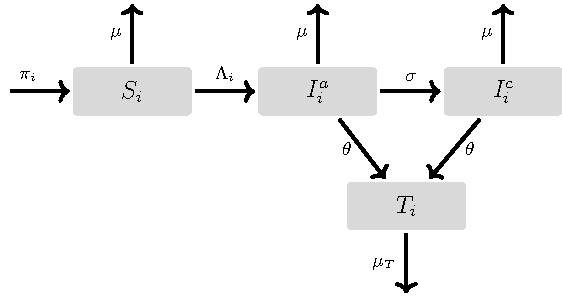
\includegraphics[width=12 cm]{Figures/Fig_S1}
	\caption[Flow diagram for the compartmental model of HIV transmission among MSM, when PrEP is not available as a prevention method]{%
	{\bf Flow diagram for the compartmental model of HIV transmission among MSM, when PrEP is not available as a prevention method}\\
	 Sexually mixing MSM are stratified in two disjoint categories according to their risk group ($i \in\{h,\ell\}$, standing for high and low, respectively). Uninfected MSM join the $i$-risk-group population at a rate $\pi_i$ and spend $1/\mu$ years selecting new sexual partners. Susceptible individuals, $S_i$, get infected with HIV at a rate $\Lambda_i$. Individuals $I^k_i$, where $k \in \{a,c\}$, with $a$ standing for acute and $c$ standing for chronic stage of infection, are infected and unaware of their infection. The progression from the acute stage of infection to the chronic stage of infection occurs at a rate $\sigma$. Infectious individuals are diagnosed at a rate $\theta$ at any stage of their infection and get immediately treated with antiretroviral therapy. Treated individuals, $T_i$, leave the sexually mixing population at a rate $\mu_T$.}
	\label{fig:FlowDiag}
\end{figure}

%% Figure S2 - Flow diagram with PrEP
\newpage
\begin{figure}[H]
	\centering
	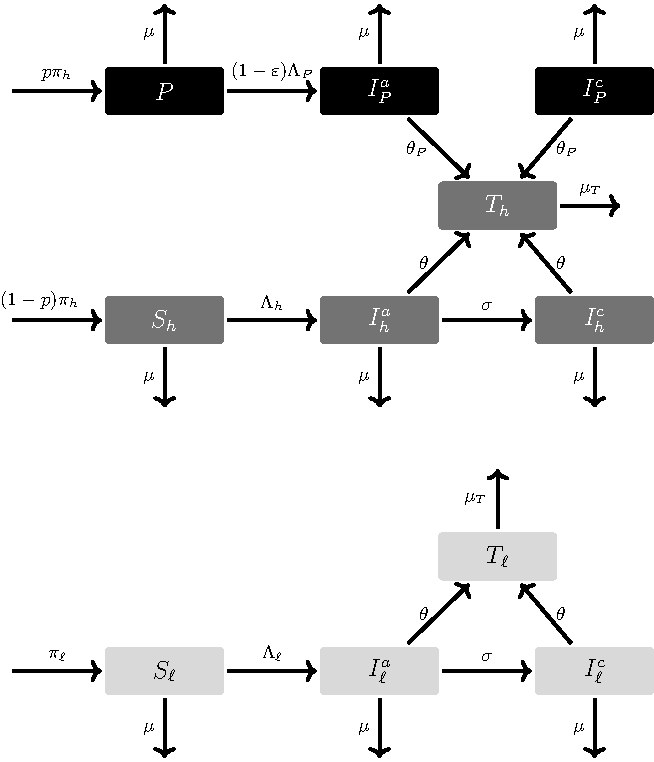
\includegraphics[width=12 cm]{Figures/Fig_S2}
	\caption[Flow diagram for the compartmental model of HIV transmission among MSM, when PrEP is available as a prevention method]{%
		{\bf Flow diagram for the compartmental model of HIV transmission among MSM, when PrEP is available as a prevention method}\\
	Dark (respectively light) gray compartments depict individuals with high (respectively low) risk of HIV infection. Only uninfected individuals at high risk of infection are eligible to adopt PrEP ($P$). PrEP users are depicted by black compartments. PrEP coverage and PrEP effectiveness are denoted by $p$ and $\varepsilon$, respectively. The HIV testing rate for on-PrEP MSM is denoted by $\theta_P$. Individuals on PrEP get infected at a rate $(1-\varepsilon) \Lambda_P$.}
	\label{fig:FlowDiagP}
\end{figure}
 
%% Figure S3 - Reproduction number & Test-and-treat effect
\newpage
\begin{figure}[H]
	\centering
	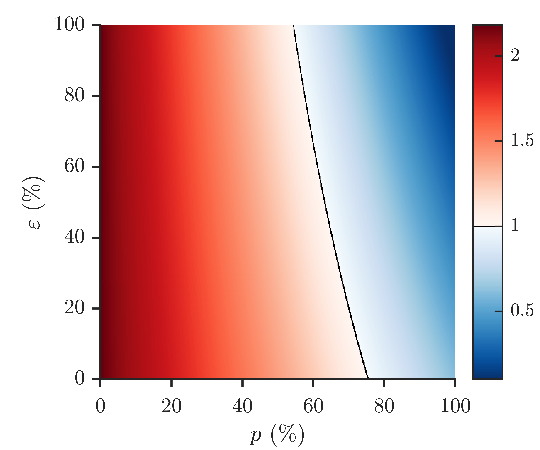
\includegraphics{Figures/Fig_S3}
	\caption[The effective reproduction number $R$ as a function of the PrEP parameters]{%
		{\bf The effective reproduction number $R$ as a function of the PrEP parameters}\\
	Color maps of the effective reproduction number, $R$, obtained for a typical parameter set calibrating our model, under the baseline scenario; i.e., high-risk MSM not on PrEP use condom with probability $30\%$, and if they get on PrEP, the probability drops at $20\%$; condom effectiveness is $70\%$. $R>1$ (i.e., epidemic persistence) is shown in red shades and $R<1$ (i.e., epidemic elimination) is shown in blue shades. The solid black line depicts $R=1$. {\bf A}  The effective reproduction number $R$ versus the PrEP coverage, $p$, and PrEP effectiveness, $\varepsilon$. {\bf B} The effective reproduction number $R$ versus the PrEP coverage, $p$, and the HIV testing rate while taking PrEP, $\theta_P$, assuming that the PrEP effectiveness is zero (i.e., $\varepsilon=0$). Note that HIV elimination is possible even when $\varepsilon=0$. This intervention is equivalent to assuming that there is no PrEP, but a fraction $p$ of the high-risk MSM get tested more frequently that the others, at a rate $\theta_P$.}
	\label{fig:R}
\end{figure}

%% Figure S4 - Voluntary PrEP coverage
\newpage
\begin{figure}[H]	
\small	
\centering		
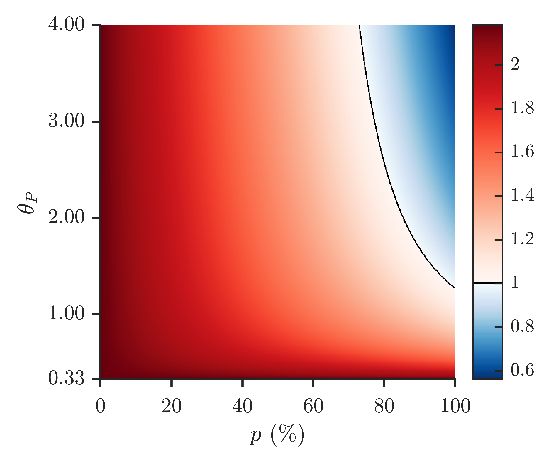
\includegraphics{Figures/Fig_S4}	
\caption[Impact of rollout with voluntary PrEP uptake, function of the relative cost of PrEP versus ART, when the PrEP effectiveness is $86\%$]{%		
	{\bf Impact of rollout with voluntary PrEP uptake, function of the relative cost of PrEP versus ART, when the PrEP effectiveness is $86\%$}\\
We illustrate the PrEP coverage ($\%$) reached voluntarily by high-risk MSM (left axis) and the endemic force of infection on high-risk MSM reached through voluntary PrEP use (right axis), assuming the PrEP effectiveness is $\varepsilon=86\%$. We assumed that (i) high-risk MSM not on PrEP use condoms with $30\%$ probability, and when they get on PrEP, the probability drops at $20\%$; (ii) condom effectiveness is $70\%$; and (iii) MSM have a fair perception of the risk of HIV infection; i.e., assumptions of the baseline scenario. The three regions correspond to the three regions identified in figure 1 of the main text. In Region~III, no MSM adopts the strategy of using PrEP (i.e., $\hat{p}(\varepsilon,r)=0$) due to high perceived cost of PrEP (i.e., $r \geq r_{\rm C}(\varepsilon)$; $r_{\rm C}$ denotes the threshold cost for epidemic control). Hence, in Region~III, there is no impact on the course of the epidemic: the endemic force of infection among high-risk MSM remains unchanged after the introduction of PrEP; i.e., $\hat{\Lambda}_h^{\rm ES}(\varepsilon, r) = \Lambda_h^{\rm ES}(0,0) = 0.07$, where $\Lambda_h^{\rm ES}(0,0)$ is the endemic incidence rate for high-risk MSM in the absence of PrEP. In Region~II,  a proportion of the population decides to use PrEP (i.e., $0<\hat{p}(\varepsilon,r) <100\%$) at the given cost, but the PrEP coverage is not enough for epidemic elimination. Hence, the epidemic is controlled and there is a reduction in the endemic incidence. Region~I, the striped area, corresponds to the case where $R\left(\hat{p}(\varepsilon,r),\varepsilon\right) \leq 1$. In Region~I, the relative cost is low (i.e., $0 \leq r \leq r_{\rm E} (\varepsilon)$), so high levels of PrEP coverage --- and thus, high levels of effective PrEP coverage (i.e., $\hat{p}(\varepsilon,r) \,\varphi(\varepsilon) \geq K$) --- are reached, and the epidemic may be averted; i.e., the endemic force of infection can be 0. In particular, for a PrEP effectiveness of $\varepsilon=86\%$, the minimum PrEP coverage $\hat{p}(\varepsilon,r)$ to reach Region~I is $K/\varphi(\varepsilon) = 56\%$.}	\label{fig:p_hat}
\end{figure}

%% Figure S5 - Risk compensation
\newpage
\begin{figure}[H]
	\centering	
	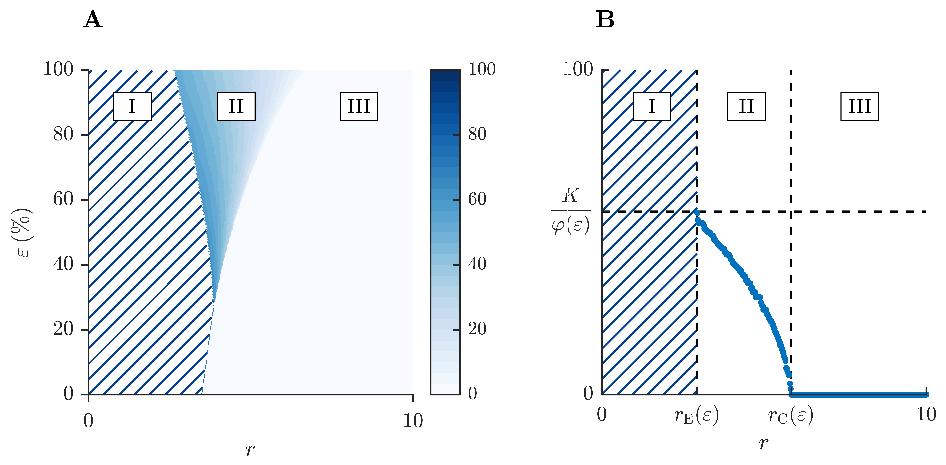
\includegraphics{Figures/Fig_S5}
	\caption[Impact of risk compensation on the voluntary PrEP coverage]{%
		{\bf Impact of risk compensation on the voluntary PrEP coverage}\\
	The voluntary PrEP coverage obtained for a typical parameter set calibrating our model, (A) assuming a complete drop in condom use among PrEP users and (B) under the baseline scenario, where condom use drops from $30\%$ to $20\%$ among PrEP users.}
	\label{fig:p_hat_CondomDrop}
\end{figure}


%%
%% 	SECION 6. REFERENCES
%%
\newpage
\renewcommand{\refname}{\section{References}}
\setlength{\labelsep}{1.5em}
\bibliographystyle{vancouver_lancethiv}
\bibliography{Bib_PrEP_HIV_SuppMat} 
\end{document}